\documentclass[11pt]{article}
\usepackage{xcolor}
\usepackage{graphicx}
\usepackage{booktabs}
\usepackage{multirow}
\usepackage[margin=1in]{geometry}
\usepackage{amsmath}
\usepackage{amssymb}
\usepackage{hyperref}
\usepackage[numbers,sort&compress]{natbib}
% Nature-style: sections with subheadings (max ~40 chars); space between paragraphs, no first-line indent
\usepackage{parskip}
\setlength{\parindent}{0pt}

\title{Logos: an evolvable reasoning engine for molecular science}
\author{\\ AI for Science (AI4S) Division @ ACE}
\date{\today}

\begin{document}

\maketitle

\begin{abstract}
The discovery and design of functional molecules remain central challenges across chemistry, biology, and materials science. While recent advances in machine learning have accelerated molecular property prediction and candidate generation, existing models tend to excel either in physical fidelity without transparent reasoning, or in flexible reasoning without guarantees of chemical validity. This imbalance limits the reliability of artificial intelligence systems in real scientific design workflows.

Here we present Logos, a compact molecular reasoning model that integrates multi-step logical reasoning with strict chemical consistency. Logos is trained using a staged strategy that first exposes the model to explicit reasoning examples linking molecular descriptions to structural decisions, and then progressively aligns these reasoning patterns with molecular representations. In a final training phase, chemical rules and invariants are incorporated directly into the optimization objective, guiding the model toward chemically valid outputs.

Across multiple benchmark datasets, Logos achieves strong performance in both structural accuracy and chemical validity, matching or surpassing substantially larger general-purpose language models while operating with a fraction of their parameters. Beyond benchmark evaluation, the model exhibits stable behaviour in molecular optimization tasks involving multiple, potentially conflicting constraints. By explicitly exposing intermediate reasoning steps, Logos enables human inspection and assessment of the design logic underlying each generated structure. These results indicate that jointly optimizing for reasoning structure and physical consistency offers a practical pathway toward reliable and interpretable AI systems for molecular science, supporting closer integration of artificial intelligence into scientific discovery processes.
\end{abstract}



\section{Introduction}

The discovery of functional molecules underpins progress across a wide range of scientific disciplines, including drug development, materials science, and energy research\cite{reymond2015chemical,vamathevan2019applications,tabor2018accelerating}. Central to this challenge is the vastness of chemical space: even when restricted to structures that obey basic chemical stability and synthetic feasibility constraints, the number of potentially accessible molecules is estimated to exceed $10^{60}$\cite{ruddigkeit2012gdb}. Within such an immense space, traditional discovery paradigms, which are largely driven by expert intuition and incremental trial-and-error, struggle to scale, increasingly limiting the pace of innovation\cite{butler2018machine,sanchez2018inverse}.

Machine learning has emerged as a powerful tool to address this challenge, enabling high-throughput prediction of molecular properties and accelerating the generation of candidate structures\cite{olivecrona2017reinvent,survey2024genai}. Deep learning architectures, particularly Transformers and graph neural networks (GNNs)\cite{gilmer2017mpnn,jensen2019gnn,you2022graph}, have established strong performance in mapping between molecular representations and physicochemical or biological properties\cite{stokes2020deep,schuster2019transfer}. These advances have substantially reduced the cost of screening and optimization for well-defined objectives. However, many real-world scientific tasks extend beyond statistical prediction or pattern matching. They require the ability to interpret abstract, often hierarchical design constraints and to translate them into concrete molecular modifications while respecting strict physical and chemical rules\cite{bilodeau2022generative,fang2023mol,m2024augmenting}.

Despite rapid methodological progress, current molecular modeling approaches remain divided along a fundamental axis\cite{survey2024llmchem}. On one side are highly specialized scientific models, such as GNN-based generators and domain-specific sequence-to-sequence architectures\cite{edwards2022molt5,schwaller2019molecular,chithrananda2020chemberta,grechishnikova2021transformer}. These models typically achieve high accuracy and chemical validity within their training distributions, but their internal decision processes are opaque. As a result, they are brittle when confronted with complex natural language instructions, novel molecular scaffolds, or competing design constraints, and they offer little insight into the reasoning behind their outputs.

On the other side are general-purpose large language models (LLMs), which exhibit strong capabilities in natural language understanding and multi-step reasoning\cite{wei2022cot,ouyang2022instructgpt}. These models can decompose complex instructions, draw analogies, and articulate intermediate reasoning steps. However, in the absence of explicit physical grounding, their application to molecular science remains limited\cite{irwin2022chemcrow,du2024molllm}. When asked to generate or modify molecular structures, general LLMs frequently produce outputs that are syntactically plausible but chemically invalid\cite{white2023assessment}, violating fundamental constraints such as valency or molecular topology. This mismatch between strong abstract reasoning and weak physical consistency presents a central obstacle to the deployment of LLMs as reliable scientific collaborators.

Together, these limitations expose a critical gap in current scientific AI systems: existing models tend to excel either at physical fidelity without reasoning transparency, or at flexible reasoning without guarantees of chemical validity. Bridging this gap is essential for enabling AI systems that can participate meaningfully in scientific design processes rather than merely generating candidate structures.

Here we introduce Logos, a compact molecular reasoning model designed to integrate multi-step logical reasoning with strict chemical consistency. Rather than pursuing scale alone, Logos aims to show that expert-level reasoning behaviour can be achieved within a controlled parameter budget when training objectives are aligned with the structure of scientific problems. The model is explicitly optimized to interpret complex molecular design instructions and to generate structures that are both chemically valid and logically traceable.

To achieve this, we adopt a staged training strategy that progressively aligns linguistic reasoning with molecular structure\cite{edwards2021text2mol,su2023moleculestm}. In the first stage, we address the scarcity of explicit reasoning data in molecular science by augmenting existing description--structure pairs with intermediate reasoning steps generated by a larger language model. These augmented examples provide the model with concrete illustrations of how abstract descriptions can be decomposed into chemically meaningful decisions. In the second stage, supervised fine-tuning\cite{ouyang2022instructgpt} aligns these reasoning patterns with molecular representations, enabling the model to follow structured instructions and to construct candidate molecules in a principled manner.

Crucially, in the final stage, chemical validity is enforced directly through a physics-guided optimization process\cite{shao2024grpo,obrien2023curriculum,horwood2023transformer}. Instead of relying solely on textual likelihoods, the model is trained using reinforcement learning objectives that incorporate chemical rules and invariants, such as those evaluated by established cheminformatics toolkits\cite{rdkit,heller2015inchi}. This stage encourages the model to favour reasoning trajectories that lead to chemically consistent structures, while systematically suppressing pathways that produce invalid molecules. As a result, chemical constraints are internalised as part of the model's generation behaviour rather than applied as an external post hoc filter.

Across multiple benchmark datasets\cite{edwards2022molt5,preuer2018fcd}, Logos achieves strong performance in both structural accuracy and chemical validity, matching or exceeding much larger general-purpose models while operating at a fraction of their scale. Beyond benchmark metrics, the model exhibits stable behaviour in multi-constraint molecular optimization tasks, where competing objectives must be balanced through iterative structural refinement. Logos exposes its intermediate reasoning steps, allowing researchers to inspect and evaluate the logic underlying each design decision.

Taken together, these results suggest that reliable scientific AI systems need not sacrifice interpretability for performance, nor physical consistency for reasoning flexibility. By jointly optimizing for logical structure and chemical validity, Logos illustrates a pathway toward AI models that function as transparent, trustworthy collaborators in molecular science. In the following sections we present the system architecture and training pipeline (Fig.~\ref{fig:framework}), benchmark results across caption-to-molecule tasks and the evolutionary training mechanism (Fig.~\ref{fig:benchmarks}, Fig.~\ref{fig:evolutionary_framework}), and the application of Logos to interactive, multi-objective molecular design (Fig.~\ref{fig:integrated_workflows}). We then discuss trade-offs, limitations, scale versus reasoning, and future work (Discussion). Full details of the task format, data preparation, supervised and reinforcement training, and bootstrapping procedure are given in Methods.
\section{Results}

\begin{figure}[htbp]
    \centering
    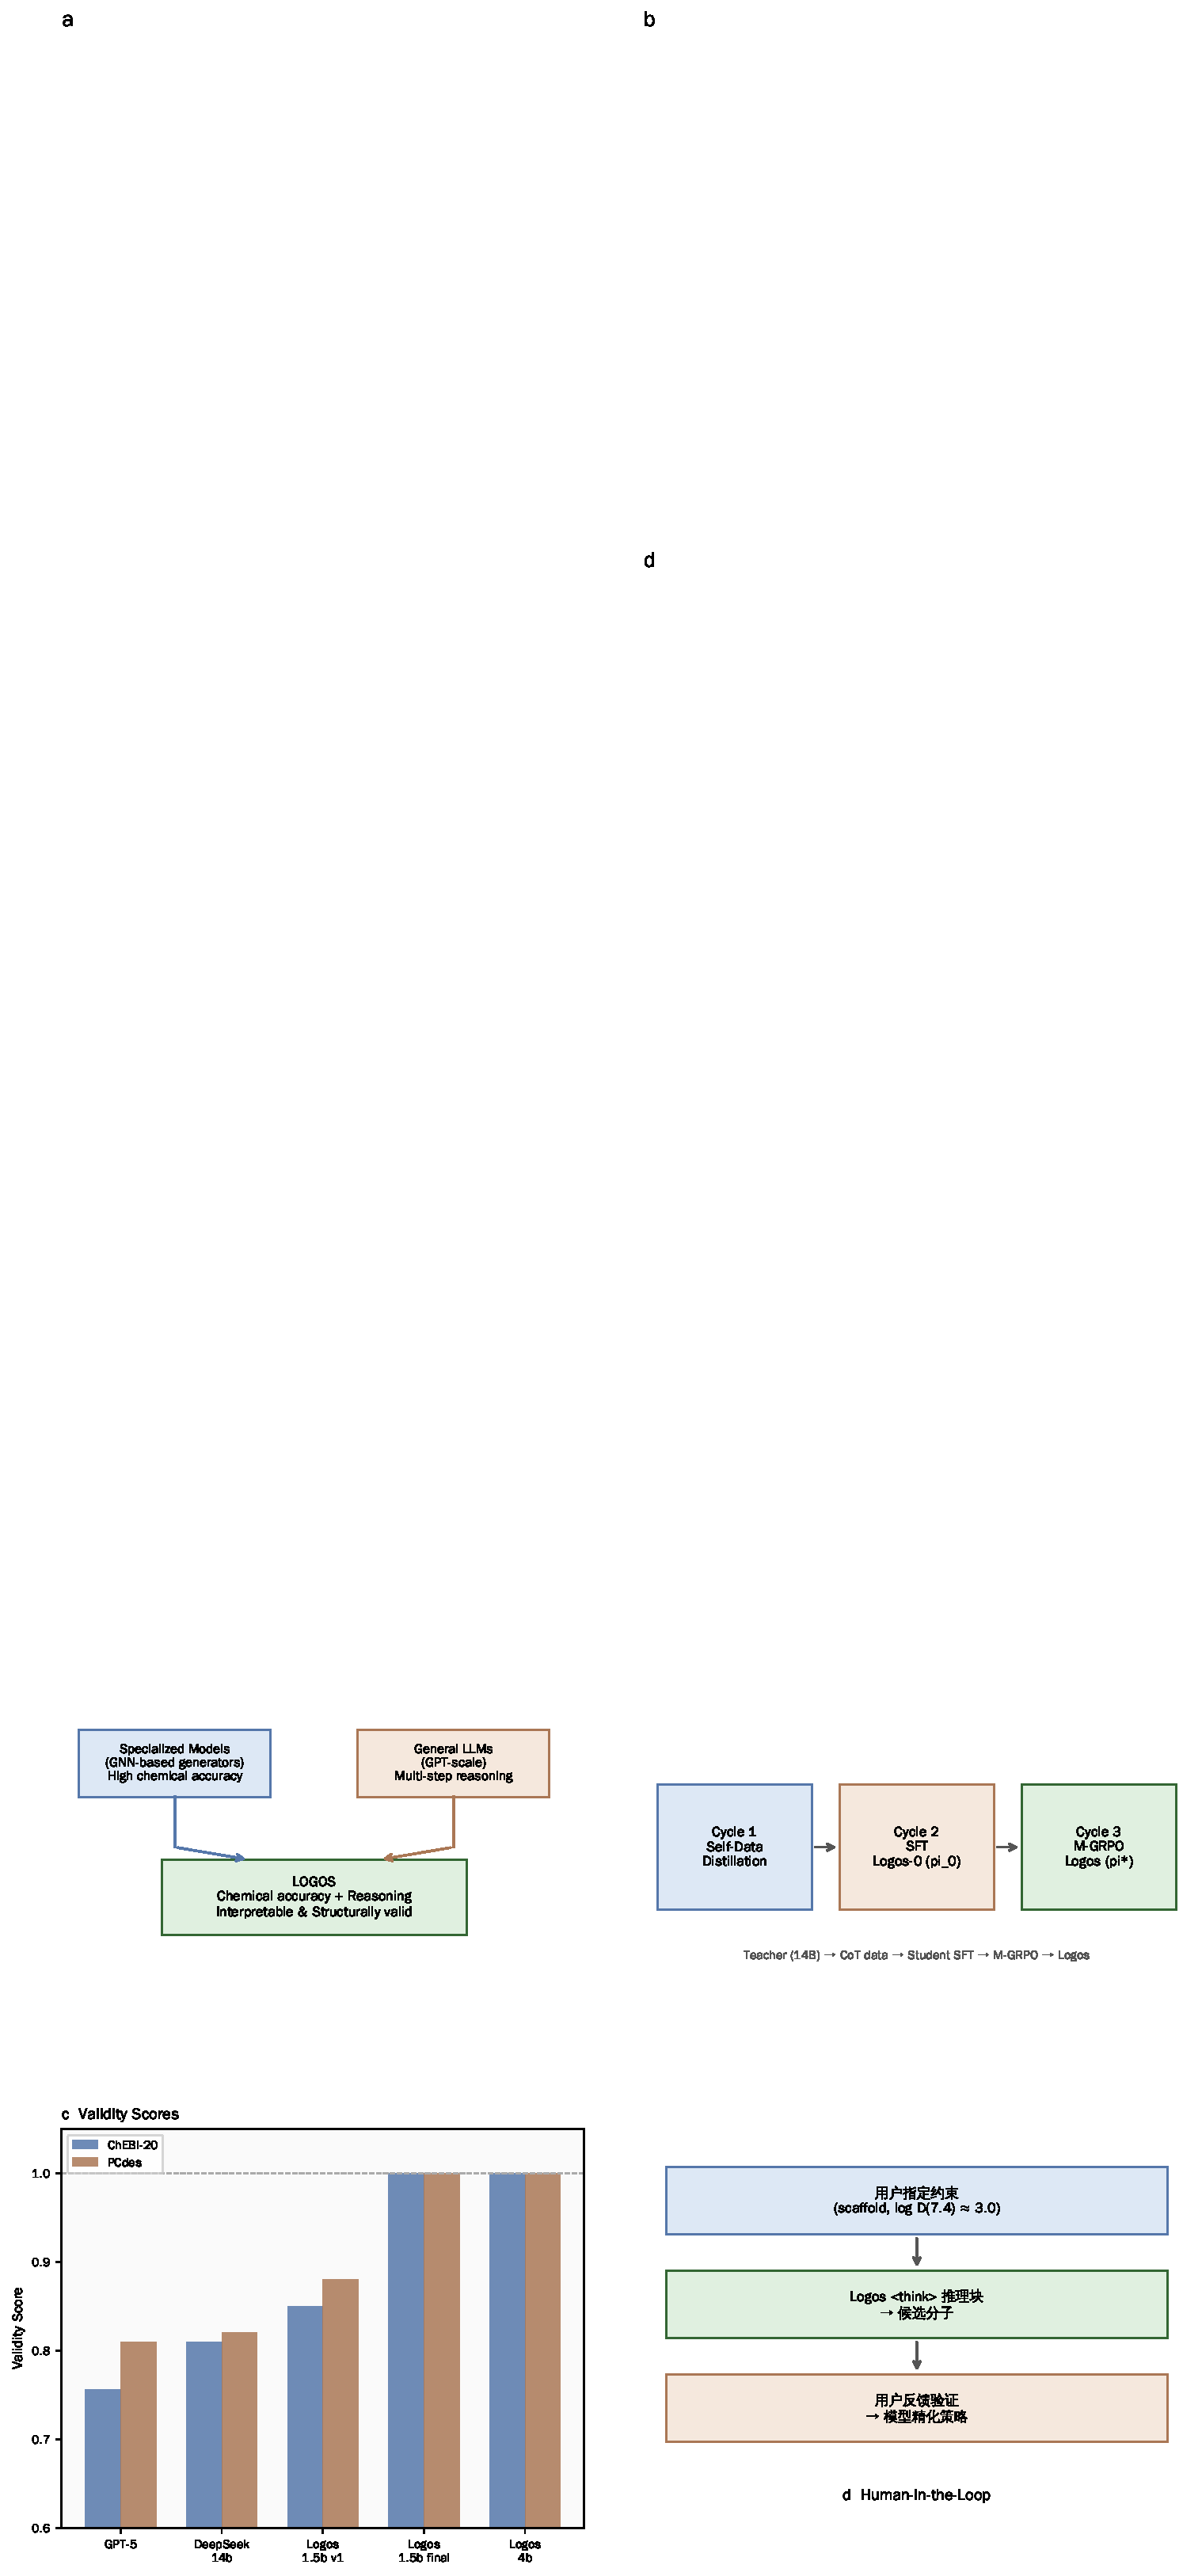
\includegraphics[width=\textwidth, height=0.675\textheight, keepaspectratio]{figures/v0/fig1.pdf}
    \caption{Conceptual framework and training pipeline of Logos. 
    \textbf{a,} Logos combines the chemical accuracy of specialized models (left) with the reasoning of general LLMs (right), addressing both interpretability and structural validity. 
    \textbf{b,} Three-stage pipeline: Cycle 1 (self-data distillation) builds chain-of-thought (CoT) data with a teacher model; Cycle 2 (supervised fine-tuning) trains on molecular design; Cycle 3 (molecule-focused GRPO) uses reinforcement learning with chemical rewards. 
    \textbf{c,} Validity scores on ChEBI-20 and PCdes; Logos-1.5b (final) and Logos-4b approach $\sim$99.9\%, outperforming larger baselines. 
    \textbf{d,} Human-in-the-loop use: the model uses its \texttt{<think>} block to refine outputs based on user feedback.}
    \label{fig:framework}
\end{figure}

\subsection{System architecture and evolutionary paradigm}

Current approaches to molecular design fall into two categories: specialized models (e.g., GNN-based generators) that achieve high chemical accuracy but lack natural language reasoning and interpretable decision paths, and general-purpose large language models (LLMs) that exhibit multi-step reasoning but frequently output chemically invalid structures because they are not grounded in valency or topological constraints (Fig.~\ref{fig:framework}a). The former are well suited to tasks where the input and output are both structural or numerical, but they do not naturally accept free-text design briefs or explain their choices in language. The latter can follow complex instructions and articulate reasoning, but when applied to molecular generation they often produce SMILES that violate basic chemical rules, limiting their use in discovery workflows where validity is required. Logos is designed to combine the chemical fidelity of specialized models with the reasoning and interpretability of LLMs, so that both the final structure and the logic leading to it can be inspected and refined.

We use a three-stage training pipeline (Fig.~\ref{fig:framework}b). In Cycle 1 (self-data distillation), a larger teacher model generates chain-of-thought (CoT) reasoning for existing molecule--caption pairs, producing a dataset that pairs descriptions with explicit reasoning steps and structures. This step addresses the scarcity of labelled reasoning data in chemistry: existing databases typically provide only caption--structure pairs, so the teacher is used to synthesise the missing reasoning layer. The student then learns to reproduce both the reasoning style and the structural output, which prepares it for the subsequent reinforcement stage where validity is explicitly rewarded. 
In Cycle 2 (supervised fine-tuning, SFT), a 1.5B-parameter student is trained on these data and becomes an intermediate model (Logos-0) that can follow instructions and output both reasoning and a molecule.
In Cycle 3 (molecule-focused group relative policy optimization, GRPO), reinforcement learning is applied with rewards that encode chemical validity (e.g., via RDKit checks) and consistency with the ground truth, so that the policy is steered toward chemically valid outputs. The third stage is necessary because SFT alone does not guarantee that the model will satisfy valency or other physical constraints at generation time; the reward signal provides a direct incentive for validity.
\textcolor{blue}{Furthermore, these three cycles operate iteratively. Through continuous looping, the original molecule--caption dataset is progressively refined and augmented with high-quality chain-of-thought (CoT) reasoning paths. To scale up our approach, a more capable 4B-parameter model is then trained on this final dataset. While the 4B model bypasses the iterative data-accumulation loops, it still explicitly undergoes both SFT (Cycle 2) and GRPO (Cycle 3) in a single, unified pass to simultaneously acquire robust reasoning and strict chemical consistency.}

On the ChEBI-20 and PCdes benchmarks\cite{edwards2021text2mol,edwards2022molt5}, the final Logos-1.5b model reaches validity scores of 0.9996 and 0.9997 respectively, \textcolor{blue}{and the Logos-4b model achieves similarly near-perfect performance} (Fig.~\ref{fig:framework}c), close to the maximum of 1.0 and above the scores of the larger baselines shown in the figure. This indicates that the GRPO stage effectively enforces chemical consistency at generation time. We report these validity results in the same figure as the pipeline overview so that readers can see both the design (panels a and b) and a first quantitative outcome (panel c) before moving to the full benchmark comparison. The same figure set also illustrates a human-in-the-loop use case (Fig.~\ref{fig:framework}d): the user specifies scaffold and property constraints; the model returns reasoning in a dedicated block and a candidate molecule; the user can supply validation feedback (e.g., from experiments or simulations), and the model uses this feedback to adjust its strategy in the next round, making the system suitable for iterative design rather than single-shot generation.

\subsection{Emergent precision in molecular representation}

We evaluated Logos and comparison models on two caption-to-molecule benchmarks: ChEBI-20\cite{edwards2022molt5,hastings2016chebi}, which focuses on biochemical and functional descriptions, and PCdes, which focuses on physicochemical properties. The two datasets differ in the type of captions (biological role and context versus physicochemical constraints), so together they probe whether the model generalises across different kinds of molecular design tasks. We compared the full evolutionary series of Logos-1.5b (from the initial version v1 through to the final model after GRPO), \textcolor{blue}{alongside our final Logos-4b model}, with four general-purpose LLMs---DeepSeek-14b\cite{deepseek2025r1}, Qwen-32b\cite{yang2025qwen3}, DeepSeek-R1-0528 \cite{deepseek2025r1}, and GPT-5, so that we could assess both the effect of each training stage and the gap between domain-specific and general-purpose models (Fig.~\ref{fig:benchmarks}).

We report several metrics. The validity score measures the fraction of generated SMILES that satisfy basic chemical rules (e.g., valency)\cite{preuer2018fcd}. General-purpose models often score well below 1.0 on this metric; for example, GPT-5 reaches 0.7564 on ChEBI-20 and 0.8100 on PCdes. Logos-1.5b (final) reaches 0.9996 and 0.9997 on the two datasets, so that invalid structures are largely removed after the GRPO stage. Exact match (EM) measures the fraction of generations that are identical to the ground-truth molecule at the graph level. Logos-1.5b (final) achieves EM 0.3406 on ChEBI-20 and 0.3103 on PCdes, while Logos-4b model significantly boosts these to 0.5588 and 0.5047 respectively, compared with 0.2488 and 0.2873 for GPT-5. The gain from v1 to the final 1.5b model is +0.2433 (ChEBI-20) and +0.2110 (PCdes) in EM, so that both validity and structural accuracy improve along the pipeline. The evolutionary trajectory (v1 to final) shows that the largest gains in EM and validity occur after the GRPO stage, consistent with the reward signal directly shaping generation toward correct and valid structures. On PCdes, the same ordering holds: Logos (final) leads on validity and EM over the general-purpose baselines, and the fingerprint similarities again show a clear gap between the domain-trained model and the larger LLMs.

To capture partial correctness and structural similarity, we also computed fingerprint-based similarities (MACCS, RDKit path, and Morgan\cite{rdkit,preuer2018fcd}). MACCS reflects the presence of key functional groups; on ChEBI-20, Logos 1.5b (final) reaches 0.9376 \textcolor{blue}{and Logos-4b further improves this to 0.9629,} versus 0.7011 for GPT-5. RDKit and Morgan similarities (\textcolor{blue}{0.8228 and 0.7422 for Logos-1.5b (final), and an impressive 0.9038 and 0.8569 for Logos-4b,} versus 0.6185 and 0.5716 for GPT-5 on ChEBI-20) indicate that the generated molecules align well with the targets in topology and local atomic environment. The Fréchet ChemNet distance (FCD)\cite{preuer2018fcd} measures the distance between the distribution of generated molecules and a reference set of drug-like molecules in a learned feature space; a lower FCD corresponds to more realistic, drug-like distributions; we use the same metric and reference set as in prior work for comparability. \textcolor{blue}{Logos-1.5b (final) reaches FCD 0.4795 on ChEBI-20, while Logos-4b achieves an even lower FCD of 0.2868,} versus 2.8354 for GPT-5, and FCD drops sharply from v1 to the final 1.5b model on both datasets (Fig.~\ref{fig:benchmarks}). Taken together, the 4B-parameter Logos (final) outperforms the much larger general-purpose models we tested on validity, exact match, structural similarity, and distributional realism, indicating that molecule-focused training with chemical rewards can compensate for smaller scale on these tasks.
% ==========================================
% Figure 2 Place Holder
% ==========================================
\begin{figure}[htbp]
    \centering
     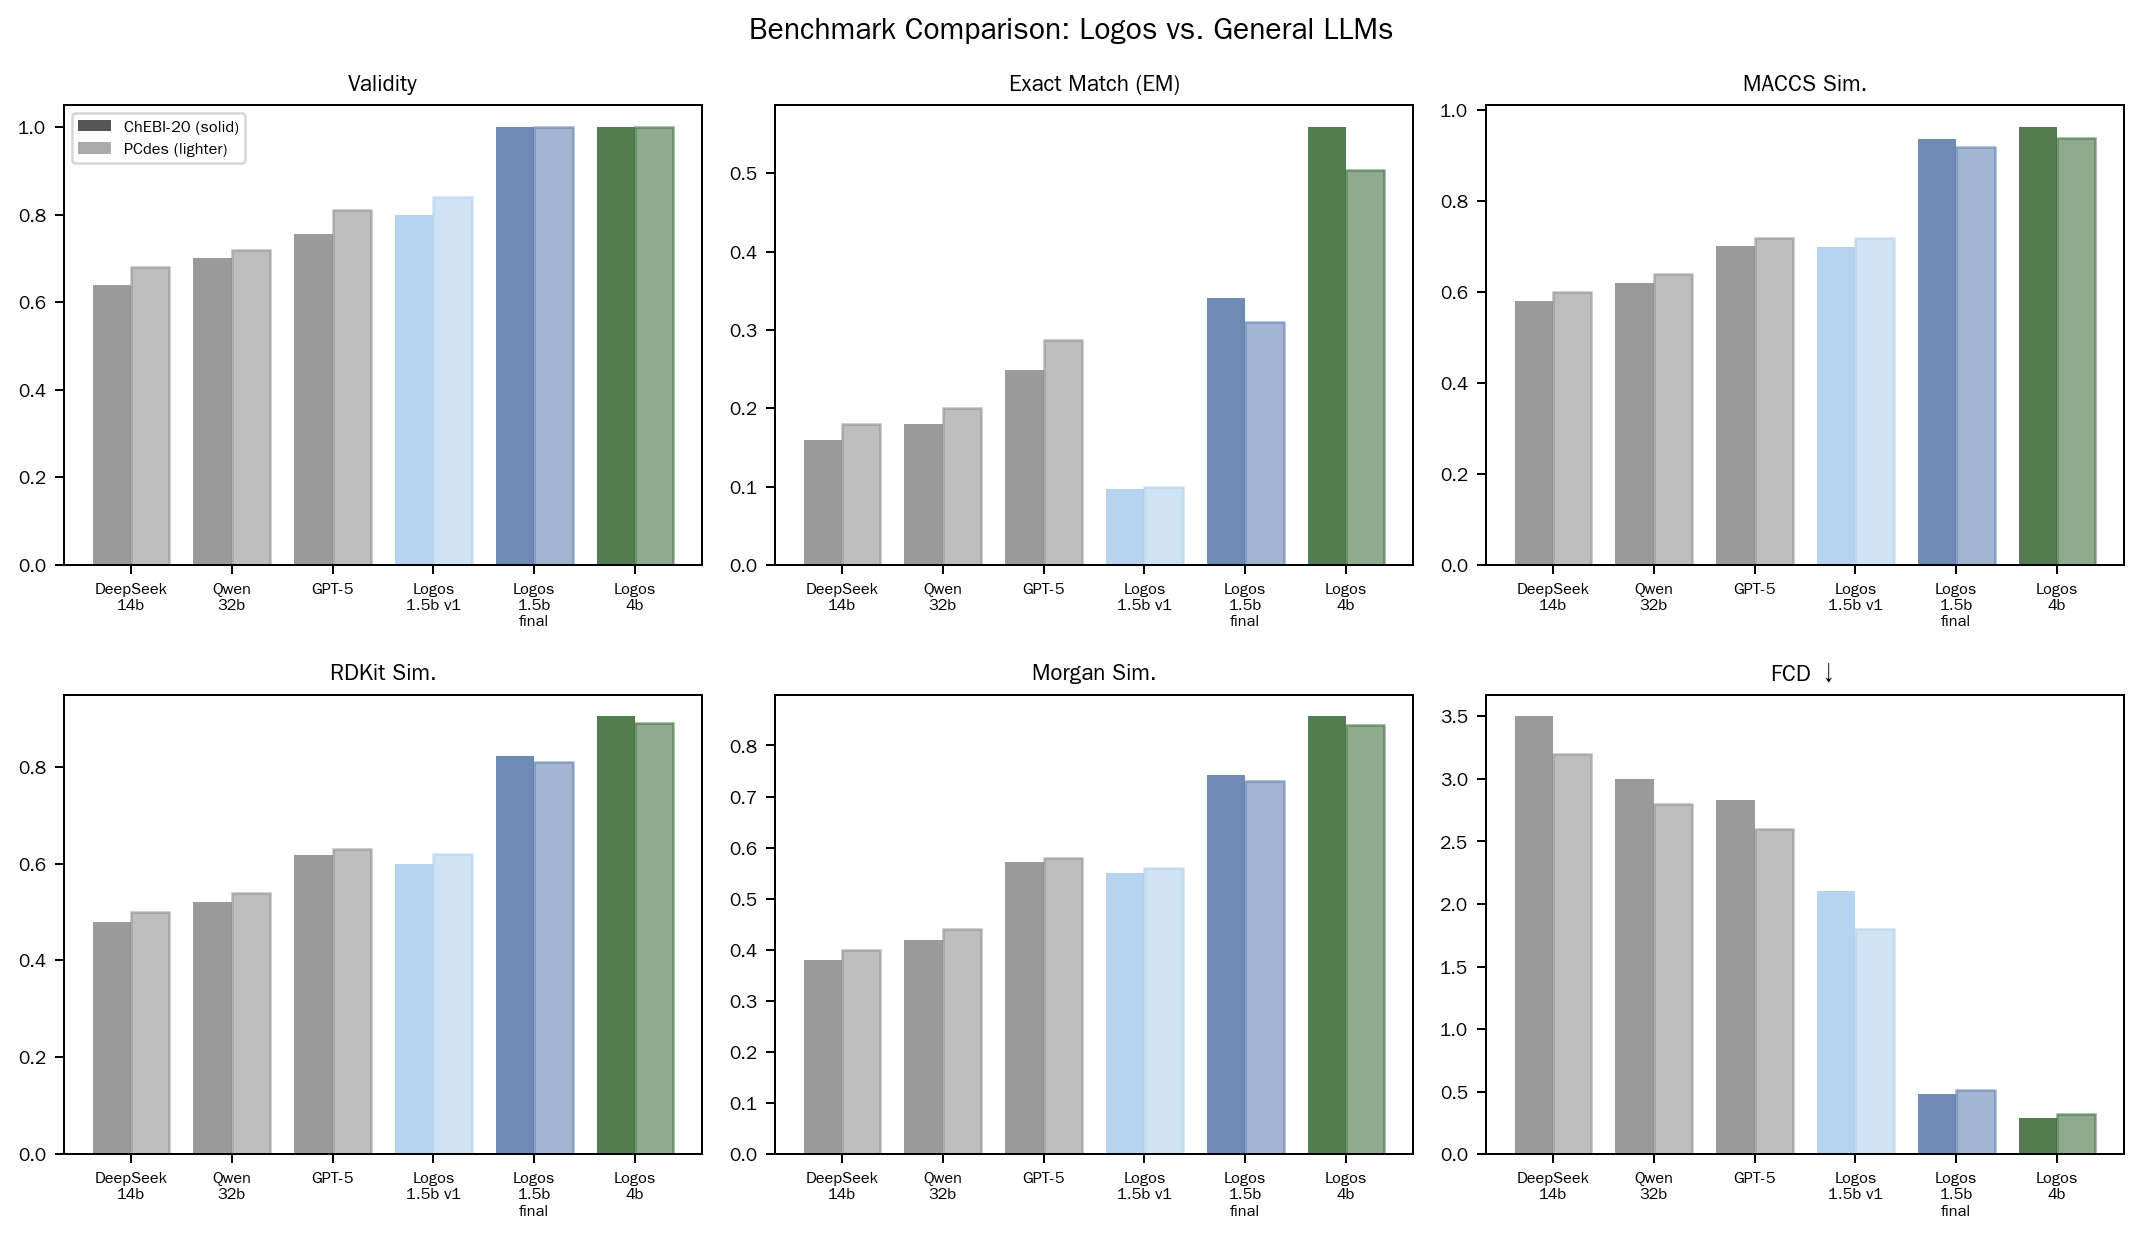
\includegraphics[width=\textwidth, height=0.75\textheight, keepaspectratio]{figures/v0/fig2.png}    
    \caption{Benchmarking across Logos-1.5b versions (v1 to final), Logos-4b and general LLMs (e.g., DeepSeek-14b, GPT-5) on ChEBI-20 and PCdes. Logos-1.5b final reaches exact match 0.3406 (ChEBI-20) and validity $\sim$1.0. Structural similarity (MACCS, RDKit, Morgan) improves across versions; FCD decreases to 0.4795, indicating that generated molecules lie closer to real drug-like chemistry.}
    \label{fig:benchmarks}
\end{figure}
\subsection{Evolutionary training mechanism and internalization of logic chain}

The training procedure is organized into three cycles that are summarized in Fig.~\ref{fig:evolutionary_framework}a. Molecular databases typically provide caption--structure pairs without explicit reasoning steps\cite{wei2022cot,edwards2022molt5,hastings2016chebi}. To obtain a training signal for reasoning, we first use a larger teacher model (14B parameters) to generate chain-of-thought (CoT) for these pairs; the teacher is prompted to explain how the description maps to structural decisions before outputting the SMILES. The resulting CoT dataset is then used to train a smaller student (1.5B/4B parameters). In Cycle 2, the student is supervised on this dataset and becomes the intermediate model Logos-0, which can follow instructions and output both a reasoning block and a molecule. Supervised training alone, however, does not guarantee that generated molecules are chemically valid\cite{olivecrona2017reinvent,ronan2024reinvent4}. In Cycle 3 we apply molecule-focused group relative policy optimization (M-GRPO)\cite{shao2024grpo}: for each prompt the model produces multiple completions; each completion receives a scalar reward that encodes chemical validity (e.g., valency checks), match or similarity to the ground truth, and structural fingerprint similarity; a KL penalty limits drift from the initial policy. The policy is updated using the relative advantage of each completion within its group, so that trajectories that yield valid, correct molecules are favoured. This stage yields the final Logos model.

Ablation experiments quantify the contribution of each stage (Fig.~\ref{fig:evolutionary_framework}b). When the full M-GRPO pipeline is used (including self-data distillation in Cycle 1), exact match on the evaluation set reaches values above 0.35. When self-data distillation is removed (M-GRPO without SDD, or SFT without SDD), performance drops to roughly 0.20--0.25, indicating that the CoT data produced in Cycle 1 are important for high accuracy. The same figure reports the evolution of maximum molecule length over training: under M-GRPO, generation length converges to a stable range, whereas the SFT-only model tends to produce longer or redundant outputs, suggesting that the reinforcement stage encourages more concise and focused reasoning. These ablations support the use of all three cycles in the final pipeline.

All training and evaluation use a fixed output format (Fig.~\ref{fig:evolutionary_framework}c). The model must first emit a reasoning block (bounded by \texttt{<think>} and \texttt{</think>} tags), then a single JSON object whose \texttt{molecule} field contains the SMILES. The system prompt defines the task and, when applicable, includes few-shot caption--molecule examples. \textcolor{blue}{For a complex request, such as generating a trisaccharide with specified glycosidic linkages, the model is expected to state the linkage logic and stereochemical constraints in the reasoning block before producing the SMILES, so that the final structure is explicitly tied to a verifiable reasoning trace.} This format allows both human inspection of the design logic and programmatic extraction and validation of the molecule (e.g., with RDKit). Enforcing reasoning-before-answer also reduces the risk of the model bypassing the reasoning step and outputting only a molecule, which would make the output harder to audit and to improve via feedback. The trisaccharide example in the figure is one instance of a task where the caption specifies connectivity (e.g., glycosidic bonds) and the model must both infer the correct topology and record its reasoning in the block before returning the SMILES.
\begin{figure}[htbp]
    \centering
    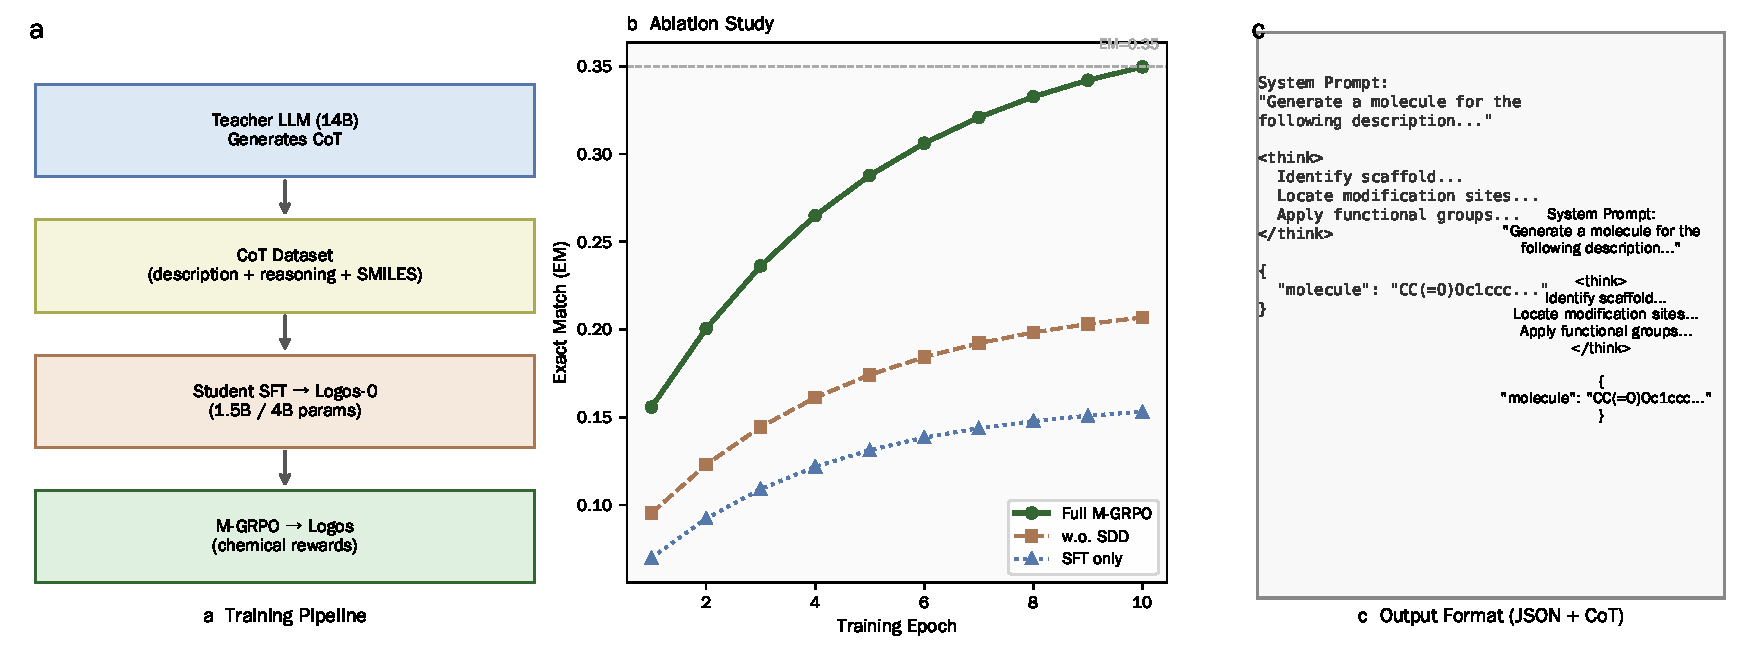
\includegraphics[width=\textwidth]{figures/v0/fig3.pdf} % Placeholder
    \caption{Evolutionary training and output format. 
    \textbf{a,} Pipeline: teacher (LLM-14B) generates CoT for description--structure pairs (Cycle 1); student (LLM-4B) is fine-tuned on CoT data to become Logos-0 (Cycle 2); M-GRPO with chemical rewards yields Logos (Cycle 3). 
    \textbf{b,} Ablations: full M-GRPO (solid blue) reaches EM $>$ 0.35; removing self-data distillation (w.o. SDD) lowers performance; M-GRPO stabilizes generation length. 
    \textbf{c,} Output format: system prompt plus JSON; the model outputs reasoning in \texttt{<think>} then the molecule in JSON, e.g. for a trisaccharide task.}
    \label{fig:evolutionary_framework}
\end{figure}
% ==========================================
% Figure 4 Caption
% ==========================================
\begin{figure}[htbp]
    \centering
    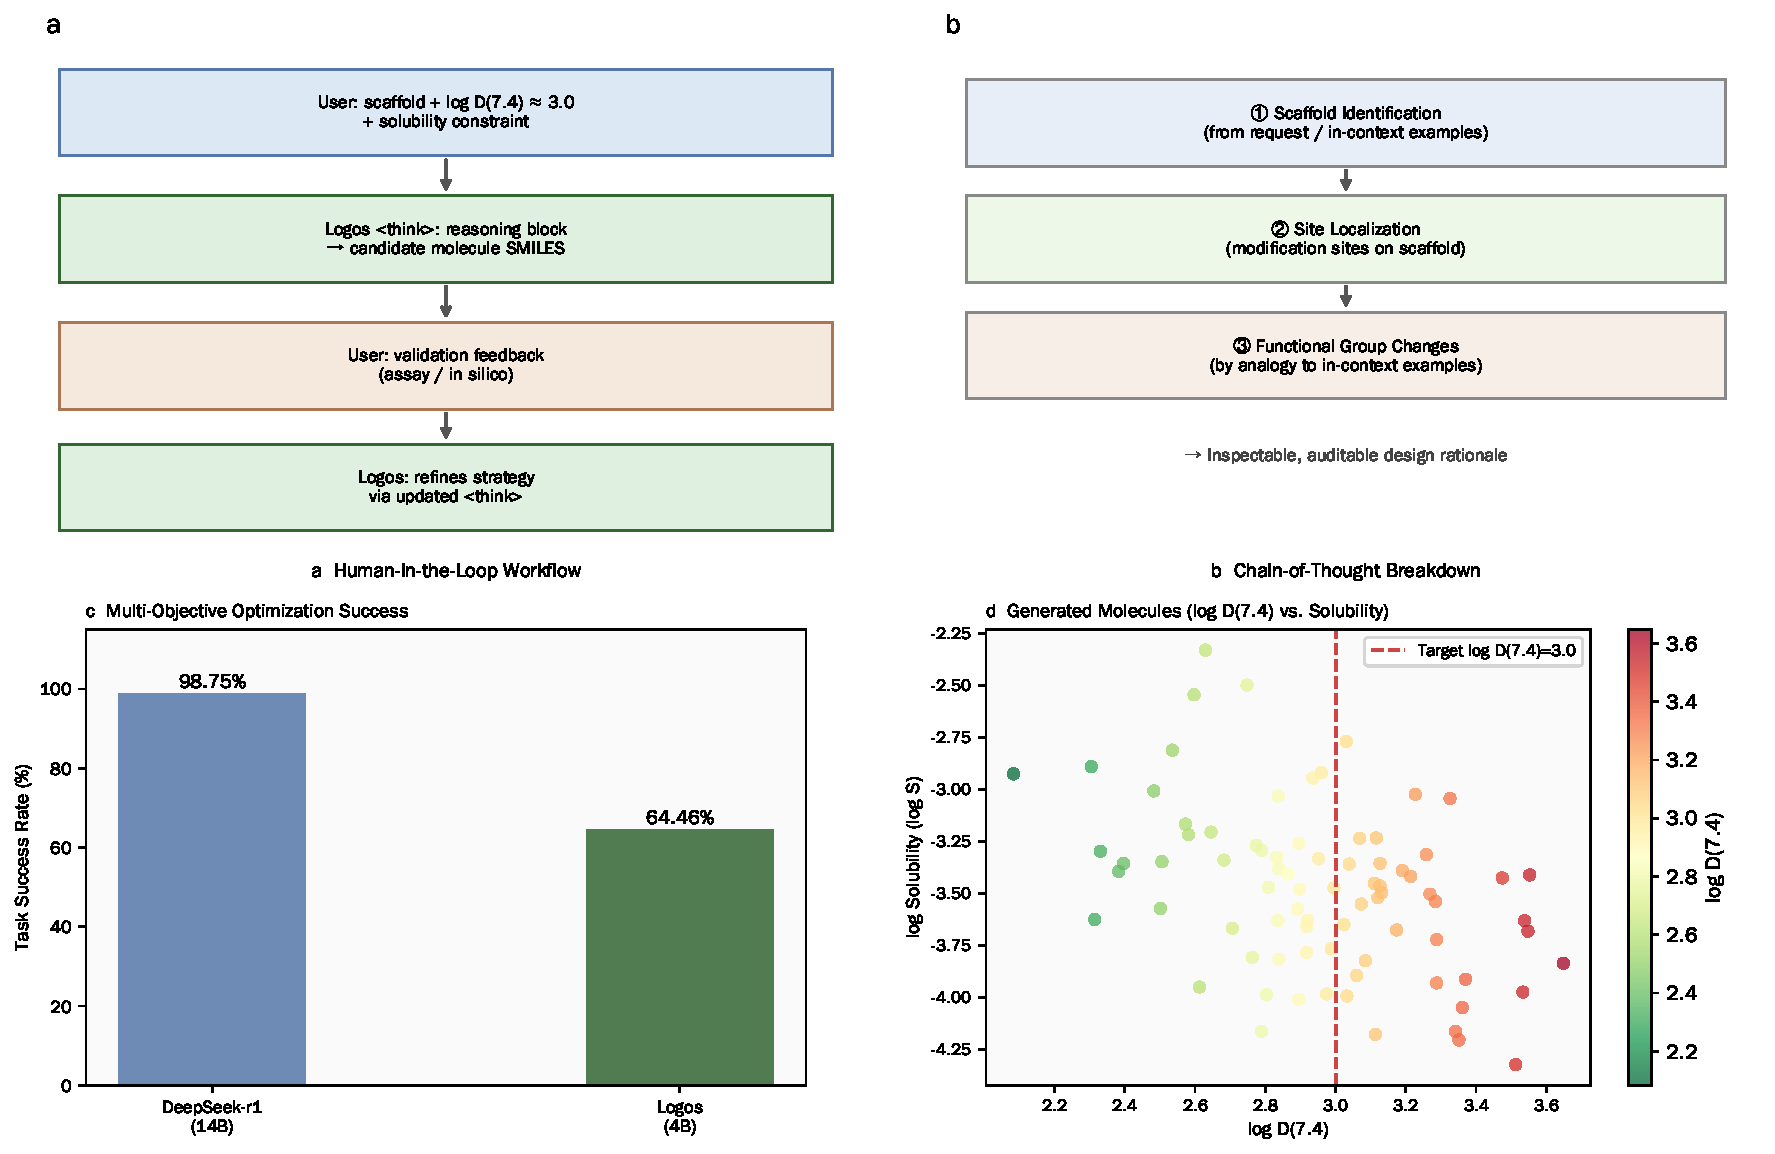
\includegraphics[width=\textwidth]{figures/v0/fig4.pdf} % Placeholder
    \caption{Integrated discovery and multi-objective optimization. 
    \textbf{a,} Human-in-the-loop: user specifies constraints (e.g., scaffold, $\log D_{7.4} \approx 3.0$); model proposes molecules; user feeds back validation; model refines via \texttt{<think>}. 
    \textbf{b,} CoT breakdown: scaffold identification, site localization, and group modifications show that outputs follow a structured reasoning path. 
    \textbf{c,} Task success in multi-parameter optimization: DeepSeek-r1 (14B) has higher validation rate (98.75\%); Logos (4B) reaches 64.46\% with fewer parameters. 
    \textbf{d,} Generated molecules cluster near the target $\log D_{7.4}$ under solubility and scaffold constraints.}
    \label{fig:integrated_workflows}
\end{figure}
\subsection{Interactive discovery paradigm and practical application}

In real-world lead optimization, chemists often iterate between design hypotheses and experimental or in silico validation, with multiple objectives (e.g., target $\log D_{7.4}$, solubility, scaffold retention) that may conflict\cite{waring2010lipophilicity,d2012multi}. We tested Logos in this setting using a human-in-the-loop protocol and compared it with a larger general-purpose reasoning model (Fig.~\ref{fig:integrated_workflows}). We chose $\log D_{7.4}$ and solubility as exemplar constraints because they are commonly used in drug discovery and can conflict with one another (e.g., increasing lipophilicity may reduce aqueous solubility), so that the task requires the model to balance competing goals rather than optimize a single quantity.

The workflow is illustrated in Fig.~\ref{fig:integrated_workflows}a. The user specifies constraints: for example, retain a given scaffold, achieve $\log D_{7.4} \approx 3.0$, and reduce solubility. The model returns one or more candidate molecules together with its reasoning in the \texttt{<think>} block. The user then provides feedback (e.g., from assays or property predictions); the model uses this feedback to refine its strategy in the next round, so that generation is iterative rather than one-shot. Because the reasoning is explicit, the user can see which structural choices led to each candidate and can correct or steer the logic. This contrasts with black-box generators that output only a structure and leave the user to infer how to improve the next round.

Fig.~\ref{fig:integrated_workflows}b illustrates how the model's chain-of-thought can be decomposed into concrete steps: identification of the core scaffold from the request or from in-context examples, localization of modification sites, and application of functional group changes by analogy to the examples. This decomposition makes the design rationale inspectable and allows researchers to audit or adjust the reasoning before accepting a structure. We compared Logos (4B parameters) with DeepSeek-r1 (14B parameters) on multi-parameter optimization tasks where validity and constraint satisfaction were both required (Fig.~\ref{fig:integrated_workflows}c). DeepSeek-r1 attains a higher validation rate (98.75\%) on the evaluated prompts, whereas Logos reaches 64.46\% with roughly one-third of the parameters. Finally, we examined the distribution of generated molecules with respect to the target property (Fig.~\ref{fig:integrated_workflows}d). Under the stated constraints (scaffold, solubility, $\log D_{7.4}$), Logos's candidates cluster near the target $\log D_{7.4}$ value, indicating that the model can steer generation toward a specified region of property space even when several constraints are active. Together, these results show that Logos can be used in an iterative, human-in-the-loop workflow for multi-objective molecular design, with reasoning that is explicit and auditable.

\section{Discussion}

The results above support two main conclusions: that a compact, domain-trained model can match or exceed much larger general-purpose LLMs on caption-to-molecule benchmarks when reasoning is combined with explicit chemical constraints, and that the same model can participate in iterative, human-in-the-loop design when multiple objectives must be balanced. Here we discuss the trade-offs implied by these findings, the limitations of the current work, the relationship between scale and reasoning in molecular tasks, and directions for future work.

\paragraph{Trade-offs.}
On standard benchmarks (ChEBI-20, PCdes), Logos reaches higher validity and exact match than the general-purpose models we tested, including GPT-5. On the multi-parameter optimization tasks (Fig.~\ref{fig:integrated_workflows}c), however, a larger reasoning model (DeepSeek-r1, 14B) achieves a higher validation rate (98.75\%) than Logos (64.46\%). There is thus a trade-off between parameter scale and task success in settings where many constraints must be satisfied simultaneously. For deployment, the choice depends on the use case: when raw success rate under complex constraints is the priority, a larger model may be preferable; when deployment cost, latency, or the need to inspect and correct reasoning at each round matters, the smaller model offers an accuracy--efficiency trade-off. In iterative workflows, the ability to see and edit the reasoning before accepting a structure can reduce the number of failed rounds in practice, so that effective performance may be closer than the single-round validation rate suggests. We did not quantify this effect; it remains a natural subject for user studies.

\paragraph{Limitations.}
Several limitations should be borne in mind. First, we evaluated on two caption-to-molecule benchmarks and one multi-parameter optimization protocol; performance on other tasks (e.g., retrosynthesis, reaction prediction, or other property targets) may differ. Second, the quality of the reasoning produced by the teacher in Cycle 1 and by Logos at inference time is not directly measured; we rely on validity and structural match as proxies. Third, the model is trained and evaluated in English; captions in other languages or mixed-language settings were filtered out and are not represented. Fourth, the bootstrapping step depends on the current model being able to generate correct molecules for some previously failed prompts; if the failure rate is very high, the gain from bootstrapping may be small. Fifth, we did not compare against all existing molecular generators (e.g., diffusion or VAE-based models\cite{vignac2022digress,gomez2018automatic}) on the same benchmarks; our comparison is focused on general-purpose LLMs and on the Logos evolutionary series. Finally, the human-in-the-loop scenario was illustrated with one constraint set ($\log D_{7.4}$, solubility, scaffold); behaviour under other constraints or with different numbers of feedback rounds has not been systematically varied.

\paragraph{Scale versus reasoning.}
A recurring question in scientific AI is whether scaling model size is necessary for strong performance or whether domain-specific training can compensate for smaller scale. On the caption-to-molecule benchmarks we report, the 4B Logos (final) outperforms the much larger general-purpose models on validity, exact match, and distributional realism. This suggests that for this task, molecule-focused training with chemical rewards can offset the advantage of scale. The result is consistent with the view that general-purpose models are not optimised for chemical validity and that injecting physical constraints via the reward signal narrows the gap. It does not imply that scale is irrelevant: the teacher model used for CoT distillation is larger (14B), and the multi-parameter optimization comparison shows that the 14B baseline can achieve higher single-round success. The takeaway is that the balance between scale and domain-specific training depends on the metric and the setting. For validity and structural accuracy on standard C2M benchmarks, domain training dominates; for complex multi-constraint satisfaction in our protocol, scale still helps. Extending this comparison to other model sizes and to other scientific domains would clarify the generality of this trade-off.

\paragraph{Future work.}
Several directions follow naturally. (i) \emph{Scaling the student:} training a larger student (e.g., 7B or 14B) with the same pipeline could show whether the gains from molecule-focused training persist at larger scale and whether multi-parameter task success improves. (ii) \emph{Benchmarks and tasks:} evaluating on additional caption-to-molecule datasets, on retrosynthesis or reaction prediction, and on property-based design with explicit objectives would strengthen the evidence for generalisation. (iii) \emph{Reasoning quality:} developing metrics or human evaluations for the correctness and usefulness of the generated reasoning (rather than only the molecule) would allow the community to optimise and compare interpretability. (iv) \emph{Integration with experiments:} coupling Logos with synthesis planning or experimental feedback loops (e.g., closing the loop with assay or property data) would test its value in real discovery campaigns. (v) \emph{Bootstrapping and data:} scaling the bootstrapping phase, incorporating active learning, or curating higher-quality CoT from experts could improve data efficiency and final performance. (vi) \emph{Other modalities:} extending the format to include spectra, reactions, or other chemical representations would broaden the scope of the approach. We hope that the pipeline and the results reported here provide a basis for these and related efforts.

\section{Methods}

We implement a multi-stage pipeline that first distils chain-of-thought (CoT) reasoning from a larger teacher into a compact student, then refines the student using reinforcement learning whose rewards explicitly encode chemical validity and consistency with ground-truth structures (Fig.~\ref{fig:framework}). An optional bootstrapping step reuses the current model to generate high-quality reasoning for previously failed samples, expanding the training set without manual annotation. The three main stages, including data preparation and CoT distillation (Cycle 1), supervised reasoning training (Cycle 2), and molecule-focused policy optimization (Cycle 3), are summarised in Fig.~\ref{fig:framework}b and Fig.~\ref{fig:evolutionary_framework}. A central design principle is that a single, strict output format is used everywhere: data construction, supervised training, reward computation, and bootstrapping all assume the same structure, so that parsing and chemical validation can be applied uniformly and multiple reward terms can be combined in one reinforcement phase. Below we describe the task and output format, data construction, supervised training, the reinforcement phase with its reward design, and the bootstrapping loop; implementation details are given at the end.

\noindent\textbf{Task and output format.}

We consider the caption-to-molecule (C2M) task\cite{edwards2022molt5,edwards2021text2mol}: given a natural-language description of a molecule (e.g., physicochemical properties, functional role, or structural hints), the model must output the corresponding SMILES string\cite{weininger1988smiles}. This setting is representative of inverse design and knowledge-guided generation in drug and chemical discovery\cite{segler2018planning,survey2024genai}. A central design choice is to require the model to emit a reasoning trace before the answer: the model first produces text inside a dedicated block delimited by \texttt{<think>} and \texttt{</think>}, then a single JSON object containing the key \texttt{molecule} with the SMILES. 
% Parsing is performed by splitting the completion on the end of the reasoning block (e.g., \texttt{</think>} followed by newline), taking the second segment, and extracting the JSON; the \texttt{molecule} field is then validated and compared using RDKit\cite{rdkit} (e.g., validity, InChI\cite{heller2015inchi}, structural fingerprints). 
\textcolor{blue}{Formally, let $y$ denote the raw model completion. The parsing process is defined as a sequential extraction pipeline:
\begin{equation}
\hat{s} = \Phi(E_{\text{regex}}(a)) \quad \text{where} \quad y = [r; d; a]
\label{eq:parsing_pipeline}
\end{equation}
Here, $y$ is first split at the reasoning delimiter $d$ (e.g., \texttt{</think>\textbackslash n\textbackslash n}) to separate the reasoning trace $r$ from the raw answer segment $a$. The function $E_{\text{regex}}$ isolates the JSON payload via regular expression matching, and $\Phi$ serves as a robust string parser that yields the predicted SMILES $\hat{s}$. To ensure fault tolerance against formatting hallucinations, $\Phi$ incorporates format correction heuristics (e.g., brace and quote removal) and fallback key routing (checking \texttt{molecule}, \texttt{smiles}, etc.). Finally, $\hat{s}$ is mapped to a computational molecular graph $\hat{m}$:
\begin{equation}
    \hat{m} = \mathcal{V}(\hat{s})
\end{equation}
where $\mathcal{V}$ represents the strict chemical validation function powered by RDKit \cite{rdkit}. If $\hat{s}$ violates chemical valency rules, $\mathcal{V}$ rejects it ($\hat{m} = \emptyset$). The successfully parsed graph $\hat{m}$ is subsequently used for downstream programmatic evaluations, including InChI-based \cite{heller2015inchi} exact matching and structural fingerprint comparisons.}
This separation allows the same pipeline to (i) train and evaluate interpretable, step-by-step reasoning, and (ii) apply programmatic chemical checks and multi-term rewards to the parsed molecule. The format is used consistently in data construction, supervised fine-tuning, reward computation, and distillation, so that no separate parsing logic is needed for each stage. Using a single, strict format across the pipeline also makes it possible to combine many reward terms in the reinforcement phase: each term receives the same parsed molecule and can call the same validation and fingerprint routines, which simplifies implementation and keeps reward definitions aligned with the data contract.

\noindent\textbf{Data preparation.}

% We start from existing molecule--caption pairs drawn from chemical databases\cite{hastings2016chebi,edwards2022molt5}. Each record includes the caption, the ground-truth molecule, and optional in-context (few-shot) caption--molecule examples used to build the system prompt. For each sample, the prompt is assembled from a task description and a variable number of few-shot examples; the model is instructed to predict the SMILES for the caption in the user message, supporting both zero-shot and few-shot training and evaluation. Some records are marked according to whether a high-quality CoT and correct molecule were previously obtained (e.g., from an earlier training run or distillation pass); this marking is used later for stratified sampling in the reinforcement set.
\textcolor{blue}{We start from an existing dataset of molecule--caption pairs $\mathcal{D} = \{(c_i, m_i^*)\}_{i=1}^N$ drawn from chemical databases \cite{hastings2016chebi,edwards2022molt5}, where $c_i$ represents the natural-language caption and $m_i^*$ is the ground-truth SMILES string. Each record optionally includes a set of $K$ in-context (few-shot) examples $E_i = \{(c_k, m_k)\}_{k=1}^K$ (where $K \ge 0$) used to build the system prompt. For each sample, the full input prompt $x_i$ is assembled by concatenating a fixed task description $\mathcal{T}$, the few-shot examples $E_i$, and the target caption $c_i$ in the user message, which can be formalized as $x_i = [\mathcal{T}; E_i; c_i]$. This formulation inherently supports both zero-shot ($K=0$) and few-shot ($K>0$) training and evaluation. Furthermore, each record is assigned a success indicator $q_i \in \{0, 1\}$ denoting whether a high-quality reasoning trace (CoT) and a correct molecule were previously generated for $c_i$ (e.g., from an earlier training run or distillation pass). The tuple $(K, q_i)$ serves as the condition variable for stratified sampling when constructing the reinforcement learning set later.}

% For supervised reasoning training, we retain only samples that already have a high-quality CoT and a correct molecule, and we filter out reasoning traces that contain non-English characters. Each training example is a triple: system (task plus few-shot examples), user (target caption), and assistant (reasoning block followed by JSON with the ground-truth molecule). This yields the CoT dataset used to train the student.
\textcolor{blue}{For supervised reasoning training, we construct a highly curated dataset $\mathcal{D}_{\text{SFT}} \subseteq \mathcal{D}$. Specifically, we retain only samples where the success indicator $q_i = 1$ (i.e., possessing a high-quality CoT $r_i$ and the correct molecule $m_i^*$), and we apply a linguistic filter to discard reasoning traces containing non-English characters. Each training example is then structured as a conversational triple $\tau_i = (p_{\text{sys}}, p_{\text{user}}, p_{\text{asst}})$, defined as follows:
\begin{equation}
     p_{\text{sys}} = [\mathcal{T}; E_i], \quad p_{\text{user}} = c_i, \quad p_{\text{asst}} = [r_i; d; f_{\text{JSON}}(m_i^*)] 
\end{equation}
where $d$ is the structural delimiter (e.g., \texttt{</think>}) and $f_{\text{JSON}}(\cdot)$ denotes the function that wraps the ground-truth SMILES into the required JSON schema. This yields the final CoT dataset $\mathcal{D}_{\text{SFT}} = \{\tau_i\}_{i=1}^{N_{\text{SFT}}}$ used to train the student model via standard autoregressive language modeling.}

% For the reinforcement phase, we construct a separate set of prompts that contain only the system and user parts (no assistant answer). Each of these is associated with the ground-truth molecule and, when applicable, the list of in-context example molecules. These fields are passed to the reward functions at training time so that each completion can be scored for validity, match to the ground truth, and whether the generated molecule is distinct from the in-context examples. Building the RL set from the same source as the SFT set (but with assistant answers omitted) keeps the two stages aligned: the model sees the same types of prompts and few-shot configurations in both supervised and reinforcement phases. To balance difficulty and few-shot configuration, we use stratified sampling: we partition samples by the number of few-shot examples and by whether the sample had previously yielded a correct CoT or not, then sample from each stratum. This ensures that the policy is trained on both easier and harder cases and across different in-context settings. We find that without this stratification, the reinforcement phase can become biased toward already-solved or single-shot prompts; with it, the model is exposed to a mix that supports few-shot-to-zero-shot generalization and more stable learning. The number of few-shot examples per sample can vary (e.g., zero, one, or several); stratifying by this number as well as by success/failure ensures that the policy is trained across the range of in-context settings that may appear at test time.
\textcolor{blue}{For the reinforcement phase, we construct a separate training set $\mathcal{D}_{\text{RL}}$ containing only the prompt contexts $x_i = (p_{\text{sys}}, p_{\text{user}})$, deliberately omitting the assistant's completion $p_{\text{asst}}$. Each prompt $x_i$ is internally coupled with a reference context $\mathcal{C}_i = (m_i^*, M_{E_i})$, where $M_{E_i} = \{m_k\}_{k=1}^K$ denotes the set of target molecules from the in-context examples. During RL training, $\mathcal{C}_i$ is hidden from the model but passed to the reward environment to evaluate the generated molecule $\hat{m}$. Specifically, the reward function scores the completion based on chemical validity, exact structural match against $m_i^*$, and generative novelty (i.e., ensuring $\hat{m} \notin M_{E_i}$). Building the RL set from the same source as the SFT set (but with assistant answers omitted) keeps the two stages aligned: the model sees the same types of prompts and few-shot configurations in both supervised and reinforcement phases.
To maintain a balanced distribution of difficulty and context length, we employ stratified sampling based on the previously defined criterion $(K, q_i)$. We partition the dataset into disjoint strata $\mathcal{S}_{K, q} = \{ x_i \in \mathcal{D} \mid |E_i| = K \land q_i = q \}$ and sample proportionally from each stratum. This explicit stratification ensures that the policy is trained across a diverse spectrum of easier ($q_i=1$) and harder ($q_i=0$) cases, as well as varying in-context settings ($K \ge 0$). We observe that without this partitioning, the RL phase tends to become biased toward already-solved or single-shot prompts. By enforcing this stratification, the model is exposed to a robust mixture that stabilizes the learning dynamics and strongly promotes few-shot-to-zero-shot generalization at test time.}

\noindent\textbf{Supervised reasoning training.}

% The student is a 4B-parameter language model that natively supports the reasoning block used for CoT. We perform full-parameter fine-tuning on the CoT dataset, maximising the likelihood of the full assistant reply (reasoning plus JSON). To encourage substantive rather than trivial reasoning, we down-weight loss on empty or very short content inside the reasoning block (consistent with training protocols for reasoning-oriented models that use a similar block structure). The maximum sequence length is set to 4096 tokens to accommodate long reasoning and large molecules. Training runs for multiple epochs over the CoT set with a standard optimiser and learning rate; we save checkpoints at regular intervals and use the final (or a selected) checkpoint as the initialisation for the reinforcement phase. This stage yields an intermediate model (Logos-0) that follows instructions and outputs both a reasoning trace and a molecule in the required format. Supervised training alone, however, does not guarantee that generated molecules are chemically valid; we therefore add a reinforcement phase that directly rewards validity and consistency with the ground truth.
\textcolor{blue}{The student policy $\pi_\theta$, initialized with a 4B-parameter language model natively supporting the CoT reasoning block, undergoes full-parameter fine-tuning on $\mathcal{D}_{\text{SFT}}$. The training objective minimizes the autoregressive negative log-likelihood of the full assistant completion $y_i$ given the input prompt $x_i$:
\begin{equation}
\mathcal{L}_{\text{SFT}}(\theta) = - \mathbb{E}_{(x_i, y_i) \sim \mathcal{D}_{\text{SFT}}} \left[ \sum_{t=1}^{|y_i|} \omega_i \log \pi_\theta(y_{i,t} \mid y_{i,<t}, x_i) \right]
\label{eq:sft_loss}
\end{equation}
To encourage substantive rather than trivial reasoning, we introduce a sample-level weighting factor $w_i$. Specifically, we down-weight the loss ($w_i < 1$) for training instances where the extracted reasoning trace $r_i$ is empty or trivially short (i.e., $|r_i| < \gamma$, where $\gamma$ is a length threshold). For instances with valid and substantial reasoning blocks, we maintain $w_i = 1$. This formulation prevents the model from exploiting length shortcuts, consistent with training protocols for modern reasoning-oriented models. The maximum sequence length is set to 4096 tokens to accommodate extensive reasoning paths and large molecular graphs. Training runs for multiple epochs over the $\mathcal{D}_{\text{SFT}}$ set with a standard optimizer and learning rate schedule. We save checkpoints at regular intervals and use the optimal checkpoint as the initialization for the reinforcement phase. This supervised stage yields an intermediate model (Logos-0) that strictly follows instructions and outputs both a reasoning trace and a molecule in the required format. Supervised training alone, however, does not guarantee that generated molecules $\hat{m}$ satisfy chemical valency constraints; we therefore cascade this with a reinforcement phase that directly rewards absolute validity and consistency with the ground truth.}

\noindent\textbf{Molecule-focused reinforcement learning.}

To align the model with chemical validity and with generalization beyond in-context examples, we use group relative policy optimization (GRPO)\cite{shao2024grpo} with rewards that are tailored to the C2M setting. For each prompt in the reinforcement set, we generate multiple completions (eight in our experiments) with the current policy at temperature 0.9. Each completion is parsed to obtain the reasoning block and the molecule field; the molecule is validated and compared to the ground truth using RDKit\cite{rdkit} and InChI\cite{heller2015inchi}. A scalar reward is computed per completion and combined with a KL-divergence penalty against the initial policy; the policy is updated using the relative advantages within each group of completions, so that trajectories that achieve higher reward are favoured.

% The reward function is a weighted combination of several interpretable terms, each of which can be computed from the parsed completion and the dataset fields (ground-truth molecule, in-context example molecules). \emph{Format and behaviour:} we reward valid JSON that contains a \texttt{molecule} key; we reward the presence of a sufficiently long reasoning block (e.g., above a minimum character length) and, importantly, we reward outputs whose molecule is \emph{not} identical to any of the in-context example molecules. This last term is intended to discourage the model from copying one of the few-shot examples and to encourage it to generalise from the task and examples to a new structure. We penalise excessively long generations to avoid runaway reasoning or redundant text. \emph{Generalisation:} we penalise reasoning text that explicitly refers to in-context examples (e.g., by mentioning ``example''), so that the model is encouraged to rely on chemical and structural reasoning rather than citing the prompt. This design directly targets few-shot-to-zero-shot generalization: in deployment, the model may see few-shot examples, but we want it to produce a distinct molecule and to justify it via reasoning rather than by repeating an example. \emph{Molecular correctness:} we give a base reward for molecules that pass RDKit validity checks and a higher reward when the generated molecule matches the ground truth (e.g., by InChI). We also use exact-match and smooth similarity (e.g., InChI-based or string similarity) between the generated and ground-truth molecule, and we add partial credit based on structural similarity computed with standard cheminformatics fingerprints (MACCS, RDKit path, and Morgan\cite{rdkit,preuer2018fcd}), so that near-correct or chemically similar outputs are favoured over invalid or unrelated ones. Together, these terms enforce format compliance, reasoning quality, chemical validity, and consistency with the ground truth while explicitly discouraging copying from in-context examples. The combination is a deliberate choice: prior work on molecular generation with reinforcement learning often optimises a single objective (e.g., validity or similarity), which can lead to format errors or to models that memorise in-context examples; here we optimise format, validity, match, and generalisation in one reward so that the policy improves on all dimensions jointly. The weights assigned to the overlong penalty, format and generalisation terms, molecular validity and match, and fingerprint similarities are chosen so that no single term dominates; in our runs we use roughly one-fifth for overlong penalty, one-third for format and generalisation, and one-half for molecular terms, with fingerprint terms sharing the remaining weight equally. This balance allows the policy to improve on chemical correctness and structural similarity without sacrificing format compliance or reasoning length.
The total reward function $\mathcal{R}_{\text{total}}$ is formulated as a weighted combination of several interpretable components, explicitly evaluating both the linguistic reasoning trace $r$ and the chemically parsed molecule $\hat{m}$ against the ground-truth $m^*$. Formally, for a given completion $y = [r; d; a]$ and a set of in-context examples $M_{E}$, the total reward is defined as:
\begin{equation}
\mathcal{R}_{\text{total}}(y_i, \hat{m}_i, m_i^*, M_{E_i}) = \sum\limits_{k \in \mathcal{K}_{\text{lang}}} \lambda_k \mathcal{R}_k(y_i, M_{E_i}) + \sum\limits_{j \in \mathcal{K}_{\text{mol}}} \lambda_j \mathcal{R}_j(\hat{m}_i, m_i^*, M_{E_i})
\label{eq:reward_total}
\end{equation}
\emph{Format and Behaviour ($\mathcal{K}_{\text{lang}}$):} We construct several heuristic rewards to enforce format compliance and reasoning quality. $\mathcal{R}_{\text{format}}$ rewards valid JSON outputs that successfully map the \texttt{molecule} key. To elicit substantive deliberation, $\mathcal{R}_{\text{cot}}$ provides a step reward if the reasoning block length exceeds a minimum threshold (e.g., $|r| > 100$). Conversely, we introduce a soft length penalty $\mathcal{R}_{\text{len}}$ to prevent runaway reasoning or redundant text. To actively discourage the policy from memorising or citing the few-shot prompts, we introduce a unified penalty $\mathcal{R}_{\text{forbid}}$. This term proportionally reduces the reward based on the occurrence frequency of reference keywords (e.g., ``example'') within the reasoning trace, and strictly assigns a zero score if the generated molecule $\hat{m}_i$ structurally matches any in-context example in $M_{E_i}$. This joint constraint directly targets few-shot-to-zero-shot generalization by forcing the model to synthesize novel structures and justify them via intrinsic chemical logic rather than prompt repetition.

\emph{Molecular Correctness and Similarity ($\mathcal{K}_{\text{mol}}$):} For the parsed molecular graph $\hat{m}$, if $\hat{m}$ is chemically valid, we compute an Exact Match reward $\mathcal{R}_{\text{EM}}$ based on strict InChI equivalence, alongside a smooth exact match $\mathcal{R}_{\text{SEM}}$ utilizing the Levenshtein ratio between the predicted and ground-truth InChI strings. Furthermore, to provide dense and continuous learning signals for near-correct structures, we incorporate structural similarity rewards:
\begin{equation}
\mathcal{R}_{\text{sim}} = \mathcal{T}(\mathcal{F}(\hat{m}), \mathcal{F}(m^*))
\end{equation}
where $\mathcal{F}$ represents standard cheminformatics fingerprint extractors (MACCS, RDKit topological, and Morgan \cite{rdkit,preuer2018fcd}), and $\mathcal{T}$ denotes the Tanimoto similarity metric. 

The weight distribution $\boldsymbol{\lambda}$ is deliberately calibrated so that the model prioritizes structural precision without neglecting formatting or reasoning integrity. In our configuration, we assign a higher weight of $0.2$ to both the exact match ($\mathcal{R}_{\text{EM}}$) and the smooth exact match ($\mathcal{R}_{\text{SEM}}$) rewards to strongly encourage convergence toward the ground-truth molecules. A uniform weight of $0.1$ is assigned to all other components, including format compliance, length penalties, anti-cheating constraints ($\mathcal{R}_{\text{forbid}}$), and fingerprint-based similarities. This balanced formulation ensures that the policy improves monotonically on chemical correctness while strictly adhering to the required JSON format and CoT reasoning style.

\noindent\textbf{Bootstrapping reasoning data from failed samples.}

Many database samples lack a high-quality CoT (e.g., previous runs had not produced a correct molecule for that caption). Rather than discarding them, we use the current model to generate new completions for these prompts. We keep only completions whose molecule matches the ground truth (e.g., by InChI comparison) and write back the corresponding reasoning block and molecule to the dataset, so that the sample is then treated as having a valid CoT. The updated dataset is used again to build supervised and reinforcement batches. This bootstrapping loop enlarges the set of samples with valid CoT without manual annotation and supports the iterative improvement we observe across training turns (Fig.~\ref{fig:evolutionary_framework}). It corresponds to a form of self-distillation: the model generates and filters its own reasoning for previously failed cases, turning them into positive training examples for the next round. In practice, we run this step when a non-empty set of failed samples exists and when we wish to expand the CoT set before another SFT or GRPO run. The write-back stores both the reasoning block and the JSON answer for each accepted completion, so that the record can be used as a full supervised example in the next data preparation pass. This closes the loop between training and data: the model improves the dataset, and the improved dataset is then used to train the model again.

\noindent\textbf{Implementation.}

Supervised fine-tuning and GRPO are implemented with the ms-swift framework; batch generation uses vLLM. Chemical validation and fingerprint computation use RDKit\cite{rdkit}. Reward terms are implemented as plugins that receive the ground-truth molecule and in-context example molecules from the dataset, so that each term can compute its contribution from the same parsed completion and data fields. No reward term requires a different parsing convention; all use the same split-on-reasoning-block and JSON extraction step, which keeps the pipeline maintainable and the reward weights comparable. For the supervised stage we use full fine-tuning with the reasoning-block loss scaling described above, maximum length 4096, and standard optimiser and learning-rate settings. For GRPO we use eight completions per prompt, temperature 0.9, and fixed weights for the reward components: roughly one-fifth for overlong penalty, one-third for format and generalisation terms, and one-half for molecular validity and match; the three fingerprint similarity terms receive equal weight. We apply an overlong filter so that excessively long generations are discarded before reward computation, and we use a KL penalty (epsilon in the GRPO update) to limit policy drift. Training is run on multi-GPU nodes in bfloat16 mixed precision. The same dataset schema (caption, ground-truth molecule, few-shot examples, and success/failure marking) is used for data preparation, SFT data export, RL data export, and bootstrapping, so that the entire pipeline can be run from a single data source and a small set of configuration parameters. The initial policy for GRPO is the checkpoint produced by the supervised stage (Logos-0), not the base language model; this ensures that the reinforcement phase starts from a model that already outputs the correct format and reasonable reasoning, and only adjusts the policy toward higher validity and match.


\bibliographystyle{plainnat}
\bibliography{reference}

\end{document}